\chapter{Reinforcement Learning}
\begin{quotation}
\noindent ``\emph{Tell me and I forget, teach me and I may remember, involve me
	and I learn.}''
\begin{flushright}\textbf{Benjamin Franklin}\end{flushright}
\end{quotation}

\vspace*{0.5cm}


\section{The reinforcement learning problem}
A reinforcement learning setting, as defined by Sutton and Barto \cite{suttonbarto}
sees two main components interact : the
\textbf{agent} (an entity performing actions) and the \textbf{environment}. 
The environment can be in several states which the agent
can observe. In some problems, the agent might not be able to observe the
full state of the environment (making the problem a partially observable one).  
The agent chooses actions based on its knowledge of the state of the
environment. These actions might (and often do) alter the state of the
environment, but will also generate a \textbf{reward}.  The
goal of the agent is to maximise the obtained reward.\\

With this simple setting, of which a diagram is shown in Figure~\ref{fig:rl},
we can design algorithms that can be trained to solve a huge variety of tasks
without ever having to include task-specific logic to the algorithm.\\

For example in the CartPole problem : the cart can be in several 
positions and have different velocities, and the pole has similar 
characteristics; the values of these characteristics constitute the state
of the environment. The agent has two actions at its disposal : nudge
the cart to the left, and nudge the cart to the right. 
The reward of the CartPole environment is +1 every timestep the pole is above a 
certain angle and the cart is within a certain range on the rail, 0 otherwise.


\begin{figure}[]
	\centering
	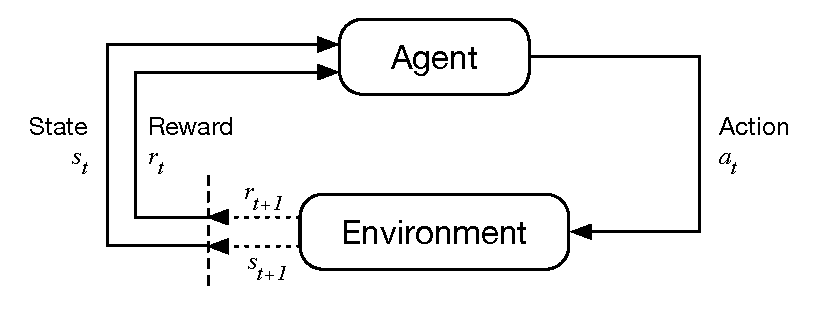
\includegraphics[width=0.65\linewidth]{fig/rl.eps}
	\caption{The setting of a reinforcement learning problem 
		\cite{suttonbarto}}
	\label{fig:rl}
\end{figure}

\subsection{Markov Decision Processes}
A reinforcement learning problem can be formally defined as a Markov 
Decision Process (MDP) \index{MDP} characterised by :
\begin{itemize}
	\item a set of states $\mathcal{S}$
	\item a set of actions $\mathcal{A}$
	\item a transition function 
		$T(s, a, s') = P(s_{t+1} = s' \mid s_t = s, a_t = a)$
	\item a reward function 
		$r(s, a, s') = \mathbb{E}
		 [r_{t+1} \mid s_t = s, a_t = a, s_{t+1} = s']$
\end{itemize}

The goal of reinforcement learning is for the agent to select, in any state it
can be in, the action that will lead it to the highest expected reward :

\begin{equation}
\label{eq:discounted_reward}
R_t = \mathbb{E}[r|\pi] = r_t + \gamma r_{t+1} + \gamma^2 r_{t+2}^2 + ... =
 \sum\limits_{i=0}^\infty \gamma^i r_{t+i}
\end{equation}

\noindent with $\pi$ the policy (see Section~\ref{sec:policy}) and 
the discount factor \index{discount factor} $\gamma \in [0, 1[$.
The discount factor allows one to tune the agent's behaviour on the
short-term/long-term spectrum. A discount factor $\gamma=0$ would mean that the
agent maximises its expected reward for the next transition only whereas a
discount factor close to one will favour behaviour that maximises long-term
reward, even if one action leads to a poor reward at first. It is chosen
by the designer as a hyperparameter for the whole length of the training.\\

\subsection{Policy}
\label{sec:policy}
\index{policy}
The agent uses a policy $\pi(a \mid s)$ which describes a probability
distribution over the action set $\mathcal{A}$, determining the probability of
selecting action each action $a_i \in \mathcal{A}$ once it is
in a certain state $s_i$. This policy is \textbf{deterministic} if and only if:
\begin{equation}
\forall\, s \in \mathcal{S},\; \exists\, a \in \mathcal{A} : \pi(a \mid s) = 1
\end{equation}
\noindent In other words : in any state, only one action can be selected.
Otherwise, the policy is \textbf{stochastic}.

\section{An example : the 2-armed bandit problem}
\label{sec:rl_example}
The 2-armed bandit setting defines two actions that the agent can perform,
each of which associated with one arm. Each arm has an underlying reward
distribution -- for the sake of this example, let us define each arm with the
following Bernoulli distributions: \index{Bernoulli}

\begin{table}[H]
	\centering
	\begin{tabular}{c|c}
		Arm \#1 & Arm \#2 \\ \hline
		0.9 & 0.1
	\end{tabular}
\end{table}

\noindent This means that arm \#1 will generate a reward of 1 with a probability
of 0.9 and arm \#2 will generate a reward of 1 with a probability of 0.1.\\

The careful reader will have noticed that this problem is stateless 
($\mathcal{S} = \{\varnothing\}$), meaning that the agent only perceives
rewards and no state observations.\\

Of course, before its first interaction with the environment, the agent has no
information whatsoever about the reward distribution of each arm, and the whole
idea of reinforcement learning is to look for evermore efficient ways to learn
the structure and parameters of a problem in order to maximise reward.\\

One could imagine a simple strategy like the following : play each arm 10 times,
then always play the arm with the highest average reward. This policy is
deterministic, and yields either $ \pi(a_1) = 1$ and $\pi(a_2) = 0$ or
$\pi(a_1) = 0$ and $\pi(a_2) = 1$. This could work in
our case, but might fail in cases where the distributions are much closer
(e.g. 0.45 and 0.55). What if the reward was sampled out of overlapping normal
distributions?\\

Deciding whether the following action should be used to explore the environment
and gain information about it; or to exploit the information already available
to try to maximise reward is not trivial. Exploring could make training slower
or affect the reward if our model of the environment is correct, but it is 
needed to increase the probability that we have indeed a correct model. This
tradeoff is called the exploration/exploitation tradeoff. \index{exploration}
\index{exploitation}\\

Sutton and Barto \cite{suttonbarto} propose two
simple ways to tackle this tradeoff : $\epsilon$-greedy and softmax selection.
Both methods fall within the denomination of Action-Value methods, meaning
that a value will be attributed to each action based on how well it did
in the past. Suppose action $a$ has been chosen $K_a$ times before timestep
$t$, and the agent has received rewards $r_1$, $r_2$,... while playing it. 
The value of action $a$ is:
\begin{equation}
Q_t(a) = \frac{r_1 + r_2 + ... + r_{K_a}}{K_a}
	\label{eq:action-value}
\end{equation}

\subsubsection{$\epsilon$-greedy}
This strategy keeps an average of the reward of each earm and chooses the next
action the following way:
\begin{equation}\begin{cases}
	\text{$a$ with $\max\limits_aQ_t(a)$} & \text{with probability } (1-\epsilon) 
	\\
	\text{random $a$} & \text{otherwise}
\end{cases}
\label{eq:egreedy}
\end{equation}
A high $\epsilon$ forces the agent to explore more, while a low $\epsilon$
allows for more exploitation of the agent's knowledge of the problem. 
$\epsilon$ is a hyperparameter of the agent, meaning that it will have to
be chosen by the designer depending on the problem and its parameters to 
strike an optimal balance between exploitation and exploration.

\subsubsection{Softmax selection}
Instead of selecting the best action with a given probability, the 
softmax selection method defines a distribution probability over the whole
action space $\mathcal{A}$. This is usually done by using a Boltzmann distribution
(also called a Gibbs distribution):
$$ \frac{e^{Q_t(a)/\tau}}{\sum_{i=1}^{n}e^{Q_t(i)/\tau}} $$
which defines the probability of selection for each action. $\tau$ is called
the \textit{temperature} parameter. A high temperature smooths the distribution,
making all actions more equally likely to be selected, and a low temperature
will tend to behave more like greedy action selection.

\section{Neural networks for reinforcement learning}
As hinted at previously, neural networks are powerful function approximators and
have yielded impressive results in reinforcement learning. They are used either
directly as policy functions, taking a state as input and outputting a
probability distribution over the action set; or as value estimators, by 
outputting a scalar which estimates the value of states and actions related to the
estimated achievable discounted reward from those states.

\subsection{Policy gradient methods}
Policy gradient methods are rather straightforward ways of learning to solve a task.
They assume that the policy is an end-to-end block of differentiable computation
(this could be a neural network, but other function approximators work too):
$$\pi(a \mid s)$$
This means that $\pi$ takes as input the state, and outputs a probability
distribution over the whole action set $\mathcal{A}$.\\

If we just received a good reward from the environment after choosing an action
$a$ from state $s$
with respect to the policy $\pi$, we could directly change the policy to 
increase the probability of selecting $a$ when we are in state $s$. The
experienced reader might have noticed that this process is very similar to
how we performed gradient descent to improve a classifier neural network. 
Indeed, supervised learning is about increasing the probability of the correct
class when given a sample (or decreasing the probability of the wrongly
predicted class). Similarly to how class labels are backpropagated through
the differentiable function, we can backpropagate rewards.
Figure~\ref{fig:supervised_vs_pg} show the process similarity between 
supervised learning and policy gradient methods.\\


\begin{figure}
	\centering
	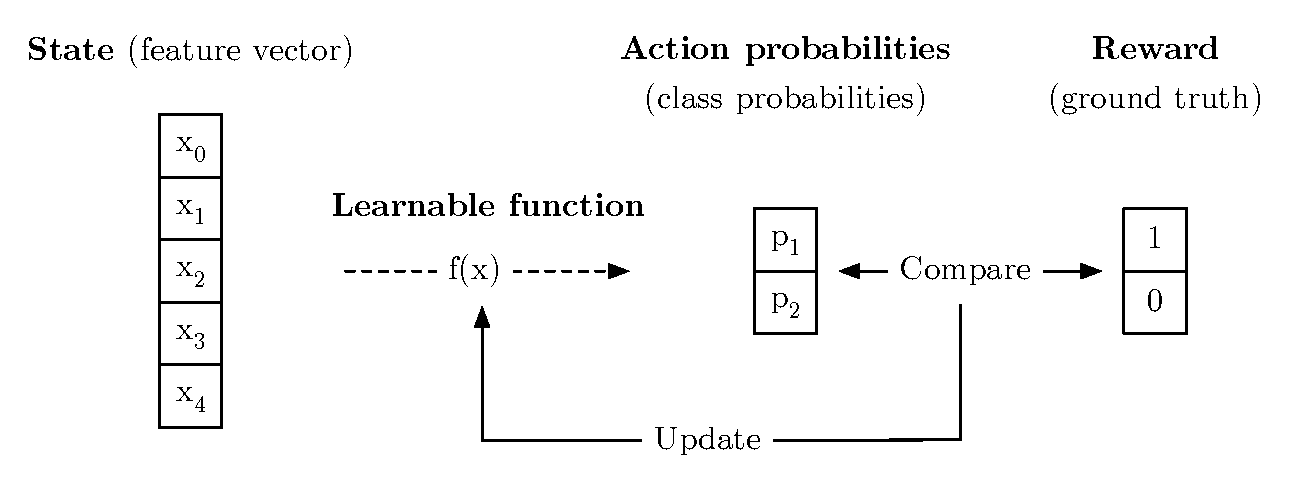
\includegraphics[width=0.8\linewidth]{fig/supervised_vs_pg.eps}
	\caption{The policy gradients process, and its similarity to
	the training process of supervised learning. Text in parentheses
	represents the supervised learning equivalent of the vectors 
	involved in policy gradients.}
	\label{fig:supervised_vs_pg}
\end{figure}

Let us assume that the
policy is defined by a neural network of which the input layer is set to 
receive an observation of the state of the environment and the output layer
defines a policy (a probability distribution over the actions set).
Training starts with a randomly initialised policy. 
When the agent performs an action chosen with its policy, the environment will
update its state and the agent will receive an observation of this state as
well as a reward signal. We can use the reward signal to proportionately
encourage (if the reward is 
positive) or discourage (if the reward is negative) taking this action in 
this specific state.\\

As the policy is defined by a neural network, we have to define a way to
update the network to find the best policy. This is done by defining a loss
function of which the gradient will be propagated back into the network, or
by defining directly the gradient as a parameters update rule.\\

Let us suppose that the agent is in a situation where it can perform two
actions, and it has received a reward of +5 after choosing action 2
sampled out of its policy $\pi(s) = [0.1, 0.9]$. We can directly use the
reward signal as a scaler for the gradient to update the network. Indeed,
multiplying the gradient of the policy $\nabla \pi(a \mid s)$ by 
$[0, 5]$ (because a +5 reward was generated by action 2) will make the network
learn what actions to perform under certain states by directly increasing the
probability of playing actions which receive a positive reward, and by
decreasing the probability of actions which receive a negative reward.\\

We can prove mathematically that multiplying the gradient of the policy
equates to the gradient of the expected reward from state $x$:
\begin{align*}
	\nabla \mathbb{E}_x[r(x)] &= \nabla \sum\limits_x\pi(x)r(x)\\
	&=  \sum\limits_x \nabla\pi(x)r(x)\\
	&=  \sum\limits_x \pi(x)\frac{\nabla\pi(x)}{\pi(x)}r(x)\\
	&=  \sum\limits_x \pi(x)\nabla\log(\pi(x))r(x)\\
	&=  \mathbb{E}_x[r(x)\nabla\log(\pi(x))]\\
\end{align*}

The method as presented still presents an issue in the sense that it only takes
into account immediate reward, but we may want to maximise long-term reward.
Let $R_t$, the discounted future reward at time step $t$ (see equation 
\ref{eq:discounted_reward}), be the metric
that we want to maximise. In a policy gradients method, we will update the
neural network policy directly with :
\begin{equation}
	\label{eq:policy_update_rule}
	\alpha \nabla \pi(a \mid s) R_t
\end{equation}
in which $\alpha$ is the learning rate and $a$ was the chosen action.

\subsection{Value methods}
There is another category of methods which use an estimate of the value of
actions or states; in other words functions which map states or state-action
pairs to estimates of their discounted future reward $R_t$. We have seen
examples of such functions previously: $\epsilon$-greedy and softmax
selection both are value-based methods (see Section~\ref{sec:rl_example} and
more specifically equation~\ref{eq:action-value}).\\

There is an important
difference between value-based methods and policy gradient methods: in the
former, the policy has to be defined by hand whereas the latter are
end-to-end (meaning that the policy is learned too). In value-based methods,
the model designer has to choose a policy that selects an action based
on estimations provided by value functions.\\

\subsubsection{V-values} 
Let us consider a problem with a relatively small set of states 
$\{s_1, s_2, ..., s_k\}$. We could estimate the \textbf{value} of 
states based on the expected discounted reward we can reach from each state, 
based on a policy $\pi$: 
$$ V^\pi(s) = R_t = \mathbb{E}
   \left[ r_t + \gamma r_{t+1} + \gamma^2 r_{t+2}^2 + ...  \right]$$
At first however, this estimate is not known. Let us imagine a problem where
only one state $s_o$ generates a reward of +100, and a state $s_{o-1}$ a state
adjacent to $s_o$. We choose to use a discount factor $\gamma = 0.9$. 
Whenever the agent plays the action that makes it go from
$s_{o-1}$ to $s_o$, the agent receives a reward of +100. Its value for $s_o$ is:
$$V^\pi(s_o) = r_t = 100$$
What about the value of $s_{o-1}$? Being right next to the goal state, it should
have quite a high value, while at the same time being lower than the goal state.
This is exactly what happens if we use our value estimation formula:
$$V^\pi(s_{o-1}) = r_t + \gamma r_{t+1} = 0+ 0.9 \times 100 = 90$$
What about a state $s_{o-2}$ adjacent to $s_{o-1}$ but not $s_{o}$? We would
compute:
$$V^\pi(s_{o-2}) = r_t + \gamma r_{t+1} + \gamma^2 r_{t+2} = 0+ 0 + 0.9^2 \times 100 = 81$$

The reader might have noticed that there is a simpler way to estimate values
than by unrolling the agent's full experience until it gets a reward. Indeed
we can, and we can use the Bellman equation to rewrite our estimation using
the values of adjacent states only by iterating on our current estimates:
\begin{equation}
V_{k+1}^\pi(s) = R_t = \mathbb{E}
   \left[ r_t + \gamma r_{t+1} + \gamma^2 r_{t+2}^2 + ...  \right] = 
   \mathbb{E}\left[ r_t + \gamma V_k^\pi(s')\right]
\label{eq:vupdate}
\end{equation}
where $s'$ is the state of highest value that can be reached from $s$. We could
rewrite this equation as the following:
$$ V_{k+1}^\pi(s) = \max\limits_a \sum\limits_{s'} p(s\mid s,a)[r(s,a,s') + 
\gamma V_{k+1}\pi(s')]$$

Iterating over estimates means that we start off with a nonoptimal value
function. It would theoretically take an infinite amount of iterations to
converge to an optimal value function $V^*(s)$, but we generally stop once the
value function changes by a small enough amount.\\

Once again, we can
use neural networks to estimate such functions. We then only have to define
a policy that decides which actions to take given these value estimates; one
example of such a policy could be a deterministic policy choosing the action
leading to the state with the highest value.\\

Equation \ref{eq:vupdate} can be used as an update rule for the $V^\pi$ network 
parametrised by its weights $\theta$ with a loss similar to :
\begin{equation}
	\label{eq:v_update_rule}
	\left[V^\pi(s\mid \theta_t) -  \left(r_t + \gamma V^\pi(s'\mid \theta_{t-1}) \right)\right]^2 
\end{equation}
\noindent which is a simple mean squared error between the estimation $V^\pi(s\mid \theta_t)$ and
the target $\left(r_t + \gamma V^\pi(s'\mid \theta{t-1}) \right)$.

\subsubsection{Q-values} 
Q-values estimate the value of state-action pairs instead of
only states; i.e. the
estimated discounted reward achievable when taking a specific action in a 
specific state. The reasoning to find an update rule is similar for V-values
and Q-values. The optimal Q function can be estimated with a Bellman equation :
$$ Q(s, a) = \mathbb{E}\left[ r_t + \gamma \max\limits_{a'} Q(s', a') \right]$$
\noindent and so can be deduced an update rule for Q networks of which the loss
can be defined with the following :

\begin{equation}
	\label{eq:q_update_rule}
\left[Q(s, a\mid \theta_t) - 
	\left( r_t + \gamma \max\limits_{a'} Q(s', a'\mid \theta_{t-1}) \right) \right]^2
\end{equation}

\subsubsection{Value networks in real life : DQN}
Estimating values using neural networks has an enormous advantage over using
tables of values. Using tables becomes intractable as the size of the state
space (or action space in the context of Q-values); worse, they become
unusable if the state space becomes continuous, unless we discretise it,
which might cause unwanted artifacts.\\

However, neural networks are not always stable, and they couldn't be used
for complex reinforcement learning tasks until Mnih et al \cite{dqn, dqn_nature}
proposed their Deep Q-network architecture. In their setting, Mnih et al. 
use the loss function described in equation \ref{eq:q_update_rule} with two
key modifications that allow the network to learn in a stable way:

\paragraph{Replay memory} Instead of updating the network using only the 
last transition that the agent went through (the tuple $(s, a, r, s')$), 
Mnih et al. sample a transition from a replay memory in which are stored
a large number of played transitions. This allows the agent to decorrelate
samples that come from the same sequence of transitions.

\paragraph{Target network} Equation \ref{eq:q_update_rule} uses a Q-value
estimate from the previous timestep as a target. This can cause oscillation
and divergence. To mitigate these effects, Mnih et al. proposed using a target
network in which the weights are copied from the network being trained 
only periodically.\\

Another key component of Mnih et al.'s architecture is the use of
convolutional neural networks \cite{convnets} which take advantage of the
relevance of spatial context in an image state. We won't delve into the
description of such networks as they won't be needed in this work.

\subsection{Actor-Critic}
We can call policy gradient methods "actor-only" methods as the methods
only choose actions without evaluating them \textit{per se}. On the other
hand, value-based methods can be called "critic-only" methods as they
evaluate possible actions and states.\\

There is a third category of methods which mixes both approaches. 
Actor-critic methods have both an \textit{actor} (the policy) and a
\textit{critic} (value functions). The actor performs the actions, and the 
critic updates the policy. One way to update the policy using a critic is to
scale the policy gradient using our current estimate of the V function:
\begin{equation}
	\label{eq:adv_update_rule}
\nabla \pi(a_t \mid s_t) (R_t - V(s_t))
\end{equation}
This way, the policy will be updated according to how wrong the critic was.
The value $R_t - V(s_t)$ is called the \textbf{advantage} \index{advantage}
because it expresses how much better (or worse) the reward was compared to 
what was estimated.


\subsubsection{The A2C algorithm}
We now have all the cards in our hand to understand the A2C
(Advantage Actor-Critic) algorithm which is a simpler version of A3C \cite{a3c}
(it only uses one thread instead of being asynchronous). 
A2C consists of a neural network
of which the input is the state $s_t$, and which outputs both a value function
$V(s_t)$ and a policy $\pi(s_t)$ (see Figure~\ref{fig:a2c}). These outputs
respectively use the updates rules described in equations \ref{eq:v_update_rule}
and \ref{eq:adv_update_rule}. The first loss function computes the error
related to the policy output:
$$ \mathcal{L}_p = \pi(a_t \mid s_t) (R_t - V(s_t))$$
and the second loss computes the error related to the value output
$$ \mathcal{L}_v = (R_{t-1} - V(s_t))^2$$
The complete loss function for the A2C agent is:
$$ \mathcal{L} = \beta_v \mathcal{L}_v + \beta_p \mathcal{L}_p $$
where $\beta_v$ and $\beta_p$ are hyperparameters used to scale both losses.\\

Algorithm~\ref{algo:a2c} shows the training
process of the A2C agent which alternates playing episodes and updating the
network according to the agent's experience.

\begin{figure}[]
	\centering
	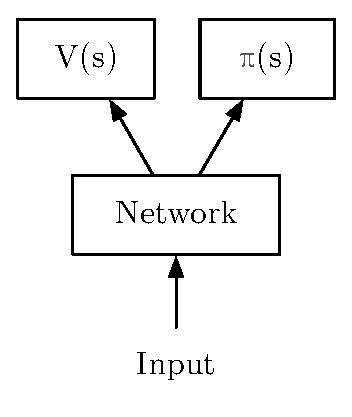
\includegraphics[width=0.2\linewidth]{fig/a3c.eps}
	\caption{The A2C network}
	\label{fig:a2c}
\end{figure}

\begin{algorithm}
\caption{The A2C training process}
\label{algo:a2c}
\begin{algorithmic}[1]
\State{$T_{\text{max}} \leftarrow$ maximum number of ticks}
\While{$T < T_{\text{max}}$}
	\Statex
	\State{\textit{// Play an episode}}
	\State{$t \leftarrow 0$}
	\While{$t <$ maximum episode length \textbf{and} episode not finished}
		\State{perform $a_t$ sampled using $\pi(s_t)$}
		\State{record reward $r_t$ and new state $s_{t+1}$}
		\State{$t \leftarrow t+1$}
	\EndWhile
	\State{$T \leftarrow T + t$}
	\Statex
	\State{\textit{// Compute advantages and gradients by unrolling episode}}
	\State{$d\theta_p \leftarrow 0$ \textit{// policy gradient}}
	\State{$d\theta_v \leftarrow 0$ \textit{// value gradient}}
	\For{$i \in \{t-1,\; t-2,\; ...,\; 0\}$}
		\State{$R \leftarrow r_i + \gamma R$}
		\State{$d\theta_p \leftarrow d\theta_p + \nabla \pi(a_i|s_i)(R-V(s_i))$}
		\State{$d\theta_v \leftarrow d\theta_v + \nabla (R - V(s_i))^2$}
	\EndFor
	\State{Update policy network using $d\theta_p$}
	\State{Update value network using $d\theta_v$}
	\Statex
\EndWhile

\end{algorithmic}
\end{algorithm}

\subsubsection{Summary}
Reinforcement learning is the study of the behaviour of an agent situated in
an environment generating rewards for the agent. Many techniques exist
to allow the agent to learn to perform well in many environments, and 
using neural networks to solve reinforcement learning problems has shown
to be very powerful.\\

We will now see how we can adapt the A2C agent to perform meta reinforcement
learning.


